\chapter{Introduction} \label{c:intro}

% http://ieeexplore.ieee.org/stamp/stamp.jsp?tp=&arnumber=6005328
% Instead, the image is dominated by speckle that is characteristic for coherent imaging. Speckle comes from the large variations in the intensity of backscattered radiation coming from the diversity in angles of the beam-target incidence, and it dominates any difference in the intrinsic reflectivity of, say, PVC pipe material, clothing, and skin.

%% RFI HSHQDC-14-00015
%% commercially available standoff - Brijot Gen 2, SET CounterBomber
%% TSA 700 AIT (advanced imaging technology) systems at 160 airports

For over thirty years the millimeter and submillimeter-wavelength spectrum has been the subject of instense interest for military and security maging applications.
The reason for this interest is that the spectral region from \SIrange{100}{1000}{\GHz} offers a good compromise between transmission through obscurant materials (favoring lower frequencies) and spatial resolution (favoring higher frequencies) \cite{kruse_why_1981}.
This interest has driven a long line of technological advancement in sources, detectors, and other technologies at these wavelengths \cite{popovic_thz_2011}.
This advancement has taken place in both ``active'' imaging, in which an observation target is illuminated by light and the reflections from that target are recorder, and `passive'' imaging, in which ambient thermal emissions are detected.

Over a similar timespan the same time the millimeter and sub-millimeter astronomical community has also been very interested in these wavelengths.
In particular, the desire to make more and more sensitive maps of the Cosmic Microwave Background (\CMB) radiation have driven this communities need for instruments capable of higher and higher sensitivies.
During the 1980's and early 1990's cooled bolometric detectors capable of achieving photon-noise-limited --- or near photon-noise-limited --- performance were developed.
By 1994 it was clear that for many astromonical applications the only way to increase sensitivity was to develop arrays of bolometers, but at that time no technology for the production of monolithic arrays was yet available \cite{richards_bolometers_1994}.

The development of voltage-biased superconducting Transition-Edge-Sensor detectors enabled the development of large-scale detector array.
These detectors are based on the use of thin superconducing films as the bolometer's themometry element, and can fabricated at large scale using standard lithographic techniques.
Their operation and advantages for array-scale operation are described in \chapterref{c:tes}.
To readout these detector arrays, several groups have developed \SQUID-based multiplexed readout systems.
This technology is now mature and is routinely deployed on both ground and balloon-borne experiements in arrays containing up to 10,000 bolometric detectors \cite{holland_scuba-2:_2013}.

The development of this technology offers new opportunities for passive imaging for security and other applications
Specifically, it is now possible to develop focal planes capable of video-rate imaging with temperature resolution of \SI{100}{\mK} or below.
This thesis decribes the design and development of the \NIST\ \Imager, a system developed to perform detection of concealed weapons at distances of \SIrange{26}{28}{\m} by producing video-rate images at \SI{350}{\GHz}.
This chapter provides an overview of millimeter-wavelength imageing and the problems that our system is intended to solve.

\section{Security Imaging}

The frequency range \SIrange{100}{1000}{\GHz} is attractive for detection of concealed weapons or contraband because many common clothing materials have hi transmission in this range \cite{bjarnason_millimeter-wave_2004}.
In general, as shown in \figref{fig:ch1-clothes-atmos-trans}, transmission through clothing steadily decreases as frequency inncreases.
This trend tends to push systems toward lower frequencies.
An example likely familiar to readers L3 Provision (correct name?) systems operating at many airports within the USA.
These are radar systems operating at ~\SI{35}{\GHz}, intended for close-range portal screening.
For applications in which is is acceptable to require individuals to pass through and pause at a particular location, these systems have excellent image quality.
Although the ProVision system only takes still images with a xxx s image acquisition time, similar portal screen systems with video-rate capabilities are also under development (xxx ref system from talk in Dresden).

\begin{figure*}
\centering
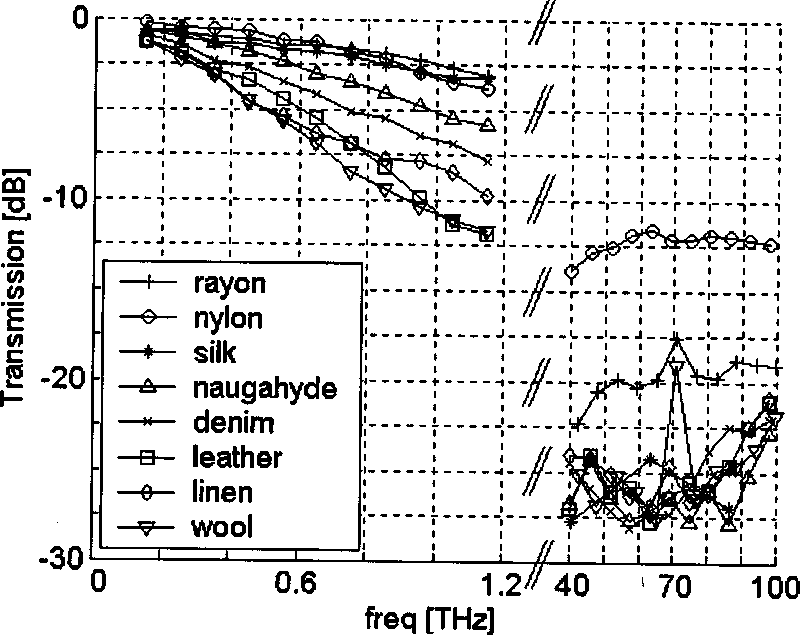
\includegraphics{drawings/ch1-clothes-bjarnason.pdf}
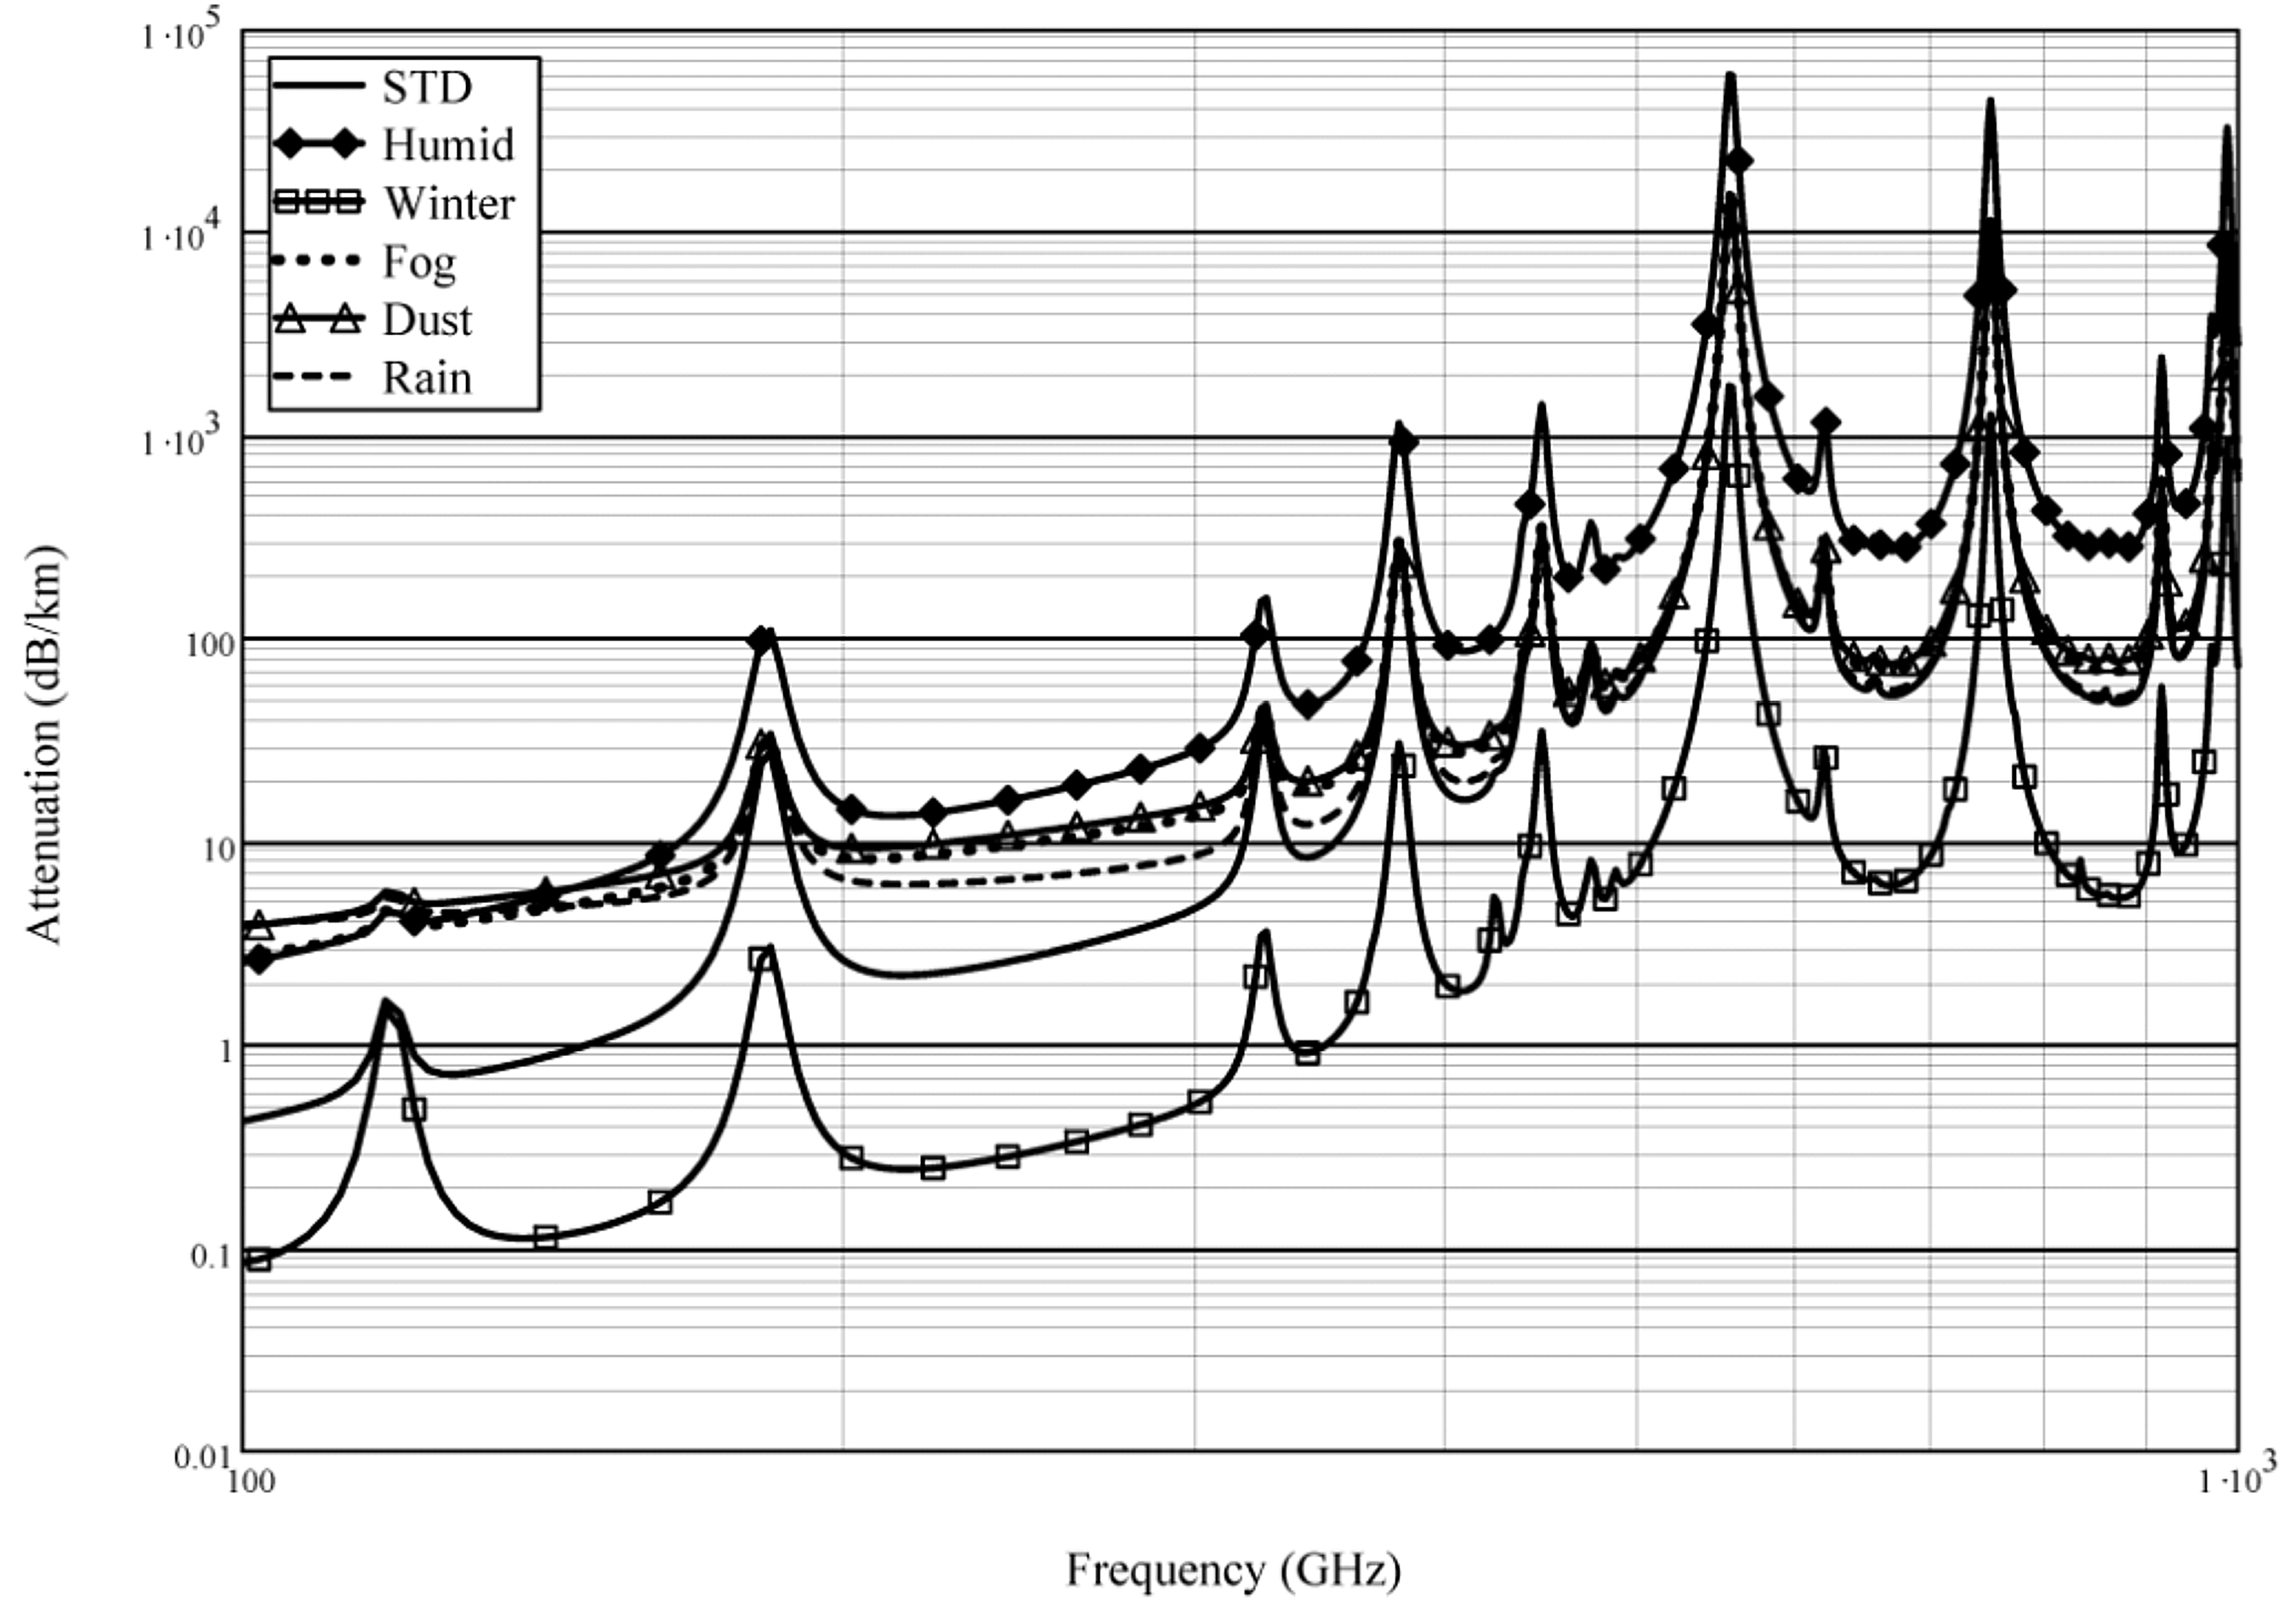
\includegraphics{drawings/ch1-atmos-trans.pdf}
\caption[Clothing and Atmospheric Transmission vs Frequency]{
  \textbf{Left}
  Plot of clothing transmission vs frequency.
  Taken from \cite{bjarnason_millimeter-wave_2004}.
  As frequency increases, transmission through all kinds of clothing decreases.
  The \SI{-10}{\dB} observation band of the \Imager\ is highlighted (\SIrange{318}{376}{\GHz}).
  \textbf{right}
  Plot showing a model of zenith atmospheric transmission on the summit of Mauna Kea, assuming \SI{0.5}{\mm} of percipital water vapor.
  The plot is illustrative only, demonstrating the presence of atmospheric transmission windows and the general trend of worse transmission at higher frequencies.
  The data was obtained using the Caltech Submillimeter Observatory (CSO) Atmospheric Transmission Interactive Plotter \cite{darek_lis_cso_????}, which is based on a published model \cite{pardo_atmospheric_2001}.
}
\label{fig:ch1-clothes-atmos-trans}
\end{figure*}

But there are other applications and operational screnarios in which portal screening systems are not feasiable.
One example is detection of suicide bomb belts, a scenario in which is it desirable to make a detection while the person being observed is some distance away.
In these scenarios it is not reasonable to expect observation targets to be stationary, so video-rate imageing is also required.
These applications are generally referred to as ``standoff'' detection because the imaging system ``stands off'' some distance from the target being imaged.
For these applications the choice of optical frequency is less clear than for portal imaging.
As shown in \figref{fig:ch1-clothes-atmos-trans}, not only does does tranmission through clothing fall with increasing frequency, but tranmission through the atmosphere does as well, although there are many atmospheric windows and line features present so that the trend is not monotonic.
Nevertheless, it is clear that lower frequencies are better for transmission through the atmosphere.

However, lower frequencies also imply worse spatial resolution for a fixed optical aperture size.
The angular resolution achievable by an aperture of diameter $D$ observing at wavelength $\lambda$ is, by the Raleigh criterion,
\begin{equation} \label{eqn:ch1-raleigh}
  \Theta \sim 1.2 \lambda / D.
\end{equation}
For portal screening this is not prohibitive. xxx how the hell does L3 Provision deal with this at 30 GHz?
But for standoff distances of \SI{10}{\m} or more, a system operating at \SI{30}{\GHz} would need an aperture of size \abt{\SI{8}{\m}} in order to achieve \SI{1}{\cm} resolution.
This strongly drives choice of frequency for standoff detection to higher frequencies.

Security imaging systems for standoff applications broadly fall into two categories: ``active'' and ``passive''.
Active systems actively illuminate the target to be images with light and use the reflected light to obtain an image.
Passive system detect thermal blackbody emmission that are naturally emitted by all objects.
Because the temperatures of objects being viewed are so low (\abt{\SI{300}{\K}}), active systems would seem to have an inherant signal-to-noise advantage over passive systems.
But the phenomenology of active imaging suffers from two problems that to-date have allowed passive imaging system to generally exceed the image quality achived with active systems.

\subsection{Active Standoff Imaging}

Both problems stem from the fact that active imaging systems use single-moded coherant sources of light, somewhat analagous to a laser point operating at visible frequencies (xxx ref Petikie).
The first problem is generally referred to as ``specular reflections''.
This refers to the fact that the intensity of light that is reflected off of the target and subsequently detected by the active imaging system is strongly dependent on the angle of the target relative to the illuminating beam.
This leads to strong highlight areas in active images which can be \SI{30}{\dB} (xxx check) or more higher than neighboring areas, making images very hard to interpret.
For a concrete example, the reader can imagine the way that sunlight at just the right angle can reflect off of the fender of another car on the road, making it difficult for thier eyes to interpret what they are looking at.

The second problem is known as ``speckle''.
When a coherant light source is diffusely reflected from a surface which varies on distance scales comparble to or larger than a wavelength, some areas of the surface will randomly be oriented more favorabley than others for reflecting light back to the system.
This leads to a random distribution of bright spots in the image known as speckle (xxx reference goodman here?).
This phenoman acts as a kind of noise in active images, and in practice the signal-to-noise ratio of active imaging systems is often limited by speckle rather than noise inherant in the detection system itself.

The active imaging community has long been aware of these issues and is working actively to address them.
One recent appraoch uses modulated multi-moded illumination to avoid these issues (xxx ref).
Another approach is to use the active system as a radar system rather than an intensity detector.
Because the radar system detects phase differences rather than intensity differences, it should in theory be less susceptible to specular reflections and speckle.

The active imaging system that at this time is closest to producing video-rate imaging largly free of specular-reflection and speckle artifacts is the 340 GHz radar system developed at JPL \cite{xxx}.
This system operates at standoff distances of \SI{16}{\m} achieving a spatial resolution of \SI{1}{\cm} at 4 frames per second.

\subsection{Passive Standoff Imaging}

Passive imaging does not suffer from the problems of specular reflection and speckle.
Rather, the primary challenge for passive imaging is implementing sufficiently sensitive detectors to achieve low-noise images at video frame rates.
One commonly used figure-of-merit for noise in a passive imaging system is the Noise Equivalent Temperature Difference (\NETD) of the image, defined as the difference in the temperature distribution at the observation target which can not be distinguished from noise in the image.
It is useful to begin with a discussion of noise in passive imaging from the perspective of bolometric detectors.

A bolometer is an optical power detector; it is senstive to the square of the incident electromagnetic field.
Bolometoer is characterized by a Noise Equivalent Power (\NEP), defined as the detected signal power equal to standard deviation of the noise in a \SI{1}{\Hz} post-detection bandwidth.
To convert the \NEP\ of the dectors to an \NETD\ for an image we must first have a conversion between detected optical power and source temperature.
For a detector sensitive to $M$ spatial modes of the electromagnetic field and with total optical effieciency $\eta_{tot}$, the optical power detected per unit optical frequency is given by the Planck law in the form
\begin{equation} \label{eqn:ch1-planck}
  P_{\nu}(\nu,T) \Delta \nu = \eta_{tot} M h \nu \frac{1}{e^{\frac{h \nu}{k_B T}} - 1} \Delta \nu,
\end{equation}
where $h$ is Planck's constant and $k_B$ is Boltzmann's constant and $T$ is the temperature of the source.
For detection of light around \SI{350}{\GHz}, and source temperatures in the range \SIrange{50}{300}{\K}, the Raleigh-Jeans approximation
\begin{equation}
  \frac{1}{e^{\frac{h \nu}{k_B T}} - 1} \approx \frac{k_B T}{h \nu}
\end{equation}
holds to within \SI{20}{\percent}, so that the total optical power in an optical bandwidth reduces to 
\begin{equation}
  P_{\nu} = \eta_{tot} M k_B T \Delta \nu.
\end{equation}
This allows us to convert a detector \NEP\ to a Noise Equivelant Temperature (\NET) via
\begin{equation}
  NET = \frac{NEP}{\eta_{tot} M k_B \Delta \nu}.
\end{equation}

To convert this detector \NET\ to an \NETD\ for an image, we make the assumptions that noise for each detector can be modeled as an uncorrelated gaussian noise source, so that the noise in for a given pixel in the image will be given by the \NET\ divided by the square root of twice the integraiton time for that pixel across all detectors\footnote{%
  xxx something about nyquist mumble mumble
}. 
We consider an image covering an area $A$ with square pixels of side length $s$, produced by an imaging system with $N$ detectors and video frame rate of $FPS$.
The integration time per pixel will then be given by
\begin{equation}
  \frac{N / FPS}{A / s^2},
\end{equation}
and so the \NETD\ of each image will be
\begin{align}
  NETD & = \frac{NET}{\sqrt{ 2 \frac{N / FPS}{A / s^2}}} \\
       & = \frac{NEP}{\eta_{tot} M k_B \Delta \nu} \frac{1}{s} \sqrt{\frac{A\,FPS}{2 N}} .
       \label{eqn:ch1-netd-defn}
\end{align}

Typical \NEP\ values for uncooled microbolometers in the millimeter-wave region are \Pnoisep{10}--\Pnoisep{100} \cite{that military report}.
In order to turn this \NEP\ into an \NETD\ we must make some assumptions.
In order to achieve sufficient spatial resoltion detecters at these wavelengths are typically sensitive to 2 modes, one per polarization, so we set $M = 2$.
We can generouslly assume one detector per image pixel, so that $\sqrt{A/N}/s = 1$.
A very good optical efficiency would be $\eta_{tot} = 0.5$, and a typical bandwidth at \SI{350}{\GHz} is \SI{35}{\GHz}.
The minimum frame rate for video imaging around 6 frames per second.
Plugging these numbers into \eqnref{eqn:ch1-netd-def} leads to an \NETD\ of \SI{50}{\K} for the best-case scenario of \Pnoisep{10} \NEP.
The maximum allowable \NETD\ for security applications is \SI{6}{\K} \cite{military}; indoors or in poor weather conditions outdoors the maximum allowable value would be smaller.
It is clear that uncooled bolometer arrays can not achieve the required performance.

A second option for room-temperature passive imaging are coherant (direct) detectors. 
Several companies have built passive imagers at xxx GHz based on this technology.

%% Keepig the following for now, because I don't really believe it,
%% and it certainly oversimplifies matters. Near-IR bolometers are viewing the peak of the
%% 300 K blackbody spectrum, so they are not in the RJ limit, so the
%% equations above don't really apply. In particular, it's not clear
%% to me whether NETD really scales with the inverser of the optical
%% bandwidth. Maybe at some point I could think about this more
%% carefully, but for now I'm removing it from the text.
% 
% Uncooled bolometers can provide excellent images in the near IR
% A typical example is the IR-TCM HD 1024 Thermography Camera Module\footnote{Jenoptik AG, Jena, Germany}, whicih produces $1024 \times 768$ pixel images with an \NETD\ of \SI{50}{\mK} at 30 frames per second using an uncooled microbolometer focal plane array.
% But uncoooled bolometer arrays can achieve this performance in the near IR because the available optical bandwidth is much larger than what is available in the \SIrange{100}{1000}{\GHz} range.
% The IR-TCM HD 1024 detects the \SIrange{7.5}{14}{\um} range, which is an optical bandwidth of \SI{19}{\THz}, a factor of \abt{530} larger than that available to the \Imager.
% Even after reducing the number of pixels in an image to a $100 \times 100$, and the frame rate to 6 frames per second, the \NETD\ from this uncooled microbolometer system would be \abt{27} times worse at \SI{350}{\GHz} than in the near-IR.
